\section{Sortering og søking}

\subsection{Sortering}
Sortering er en av de viktigste operasjonene man har, og det brukes også mye som en del av andre operasjoner. Tenk for eksempel hvis du spiller kortspillet bridge. Da får du utdelt 13 kort, og for å ha oversikt over hvor bra hånden din er sorterer du den etter farge og kortenes valør innad i hver farge.
\\\\
Egenskaper sorteringsalgoritmer kan ha:
\begin{itemize}
    \item Sammenligning
    \begin{itemize}
        \item Tregt: O(n2)
        \begin{itemize}
            \item Bubblesort
            \item Insertion-sort
            \item Selection
        \end{itemize}
        \item Optimalt: $O(n lg n)$
        \begin{itemize}
            \item Heapsort
            \item Merge-sort
            \item Quicksort
        \end{itemize}
    \end{itemize}
    \item Ikke sammenligning
    \begin{itemize}
        \item $O(n)$
        \begin{itemize}
            \item Counting-sort
            \item Radix-sort
            \item Bucket-sort
        \end{itemize}
    \end{itemize}
\end{itemize}

\subsubsection{Stabilitet}
At en sorteringalgoritme er stabil vil si at den ikke bytter om på like elementer.

\subsection{Splitt og hersk/Divide and conquer}
%strukturell induksjon

Problemene deles opp i flere delproblemer som ligner på hovedproblemet men i mindre størrelse, og løser problemene rekursivt. Deretter kombineres løsningene for å få en løsning på det originale problemet. MERGE SORT følger denne paradigmen tett.
\\\\
Paradigmen involverer tre steg i hver grad av rekursjonen:
\begin{itemize}
    \item \textbf{Splitte} problemet opp i et antall subproblemer som er mindre instanser av det samme problemet.
    \item \textbf{Herske} over problemene ved å løse de rekursivt. Hvis subproblemenes størrelser er små nok, kan de løses rett frem.
    \item \textbf{Kombinér} løsningene sammen til en løsning på originalproblemet.
\end{itemize}

\noindent Når en algoritme inneholder et rekursivt kall til seg selv, kan vi ofte beskrive kjøretiden med en rekurrensligning.

\subsection{Sammenligningsbaserte sorteringsalgoritmer}
Dette er en av to grupper sortering. Felles i denne gruppen er at soteringen skjer ved sammenligning av to elementer. De fleste av disse metodene klarer seg med å jobbe direkte i den originale inputlisten (altså at de ikke trenger å opprette nye, midlertidige lister), og disse sies å være "in place" sorteringsalgoritmer. Sammenligningsbasert sortering har en worst-case på $\Omega(n lg n)$.

\subsubsection{BUBBLESORT}
Dette kan sies å være den enkleste og mest naive av alle sorteringsalgoritmer. Bubblesort tester to og to naboelementer, og dersom den finner at det første elementet er større enn det neste bytter de plass. Effektiv på små datamengder. Denne algoritmen bruker sammenligning, og skjer "in place".

\begin{figure}[H]
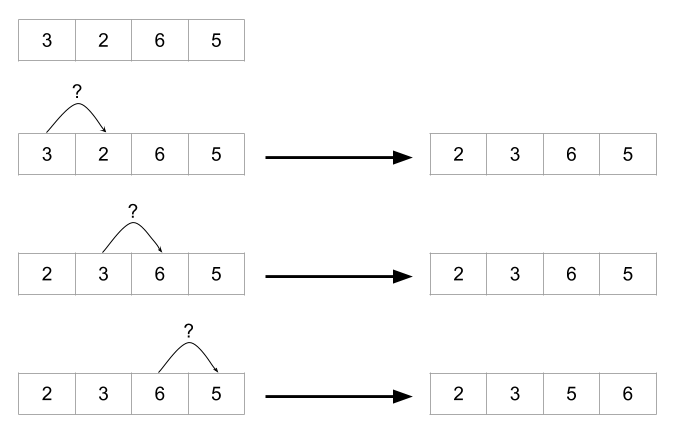
\includegraphics[scale=0.5]{images/bubblesort}
\centering %centering the image
\caption{Bubblesort}
\label{fig:bubblesort}
\end{figure}

\begin{lstlisting}
    for i = 0 to A.length - 1 do
    	for j = A.length downto i + 1 do
		    if A[j] < A[j - 1] then
		    	exchange A[j] with A[j - 1]
		    end if
	    end for
    end for
\end{lstlisting}

\begin{boxed}
Gitt tallfølgen 6, 5, 3, 1, 8, 7, 2 4. Vil sorteres slik at etter en runde vil rekken bli 5, 3, 1, 6, 7, 2, 4, 8. Neste runde vil den være: 3, 1, 5, 6, 2, 4, 7, 8. Så vil den bli: 1, 3, 5, 2, 4, 6, 7, 8. Deretter: 1, 3, 2, 4, 5, 6, 7, 8. Etter fem runder blir rekkefølgen: 1, 2, 3, 4, 5, 6, 7, 8.
\end{boxed}

\noindent Kjøretiden til Bubblesort er \textbf{$\theta(n^2$} for både gjennomsnittlig og verste tilfelle. Det er ikke så vanskelig å se for seg. Hvert eneste element kan risikere å måtte flytte seg opptil $n$ plasser under sorteringen. Boblesortering er effektiv på veldig små mengder.

\begin{table}[H]
    %\caption{}
    \label{tab:bubblesort}
    \centering
    \begin{tabular}{|L{15em} | L{15em}|}
        \hline
        \rowcolor[HTML]{303F9F}
        \textbf{\textcolor{white}{Tilfelle}} & \textbf{\textcolor{white}{}}\\
        \rowcolor[HTML]{E6E6E6}
        Best case & $\theta(n)$\\
        Average case & $\theta(n^2)$\\
        \rowcolor[HTML]{E6E6E6}
        Worst case & $\theta(n^2)$\\
        Minne & $\theta(1)$\\
        \rowcolor[HTML]{E6E6E6}
        In-place & Ja\\
        Stabil & Ja\\
        \rowcolor[HTML]{E6E6E6}
        Paralelliserbar & Nei\\
         \hline
    \end{tabular}
\end{table}

\subsubsection{INSERTION SORT}
Denne sorteringen er nok den mest intuitive av dem alle, og foregår "in place". Den tar utgangspunkt i det første elementet, og sjekker så element nummer to. Deretter settes de slik at de er sortert i forhold til hverandre. Så tar den tredje element of ser hvor dette skal plasseres i forhold til de to første. Slik fortsetter det. Når $i - 1$ elementer er ferdig sortert og det $i$'te kommer, er det riktig plass i rekken for element nummer $i$ – etter at det er satt på plass, har vi $i$ sorterte elementer, og vi kan gå videre med element $i + 1$. Dette er den måten de aller fleste sorterer en korthånd på. Insertion sort er, i likhet med bubblesort, også meget effektiv på små datamengder. 
\\\\
Kjøretiden her er også \textbf{$\theta(n^2)$} både for gjennomsnittlig kjøretid og i verste tilfelle. Men i praksis er den ofte bedre en bubblesort. Et veldig viktig poeng er: hvis du har en hel del elementer som nesten er sortert ferdig, er denne metoden helt suveren (på slutten av quicksort f.eks.). Er listen allerede sortert når Insertion sort kjøres blir kjøretiden $T(n)$.

\begin{figure}[H]
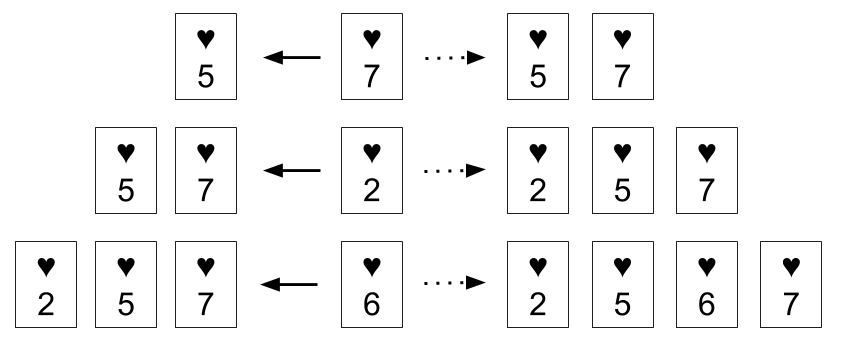
\includegraphics[scale=0.5]{images/insertionsort}
\centering %centering the image
\caption{Insertion sort}
\label{fig:insertionsort}
\end{figure}

\begin{lstlisting}
    for j = 0 to A.length do
	    key = A[j]
	    i = j - 1
	    while i > 0 and A[i] > key do
	    	A[i + 1] = A[1]
	    	i = i - 1
	    end while
	    A[i] + 1 = key
    end for
\end{lstlisting}

\begin{boxed}
Gitt tallrekken 6, 5, 3, 1, 8, 7, 2, 4. Begynner med 6, som er første tall. Ser så på 5. 5 er mindre enn 6, og flyttes til plass null. Rekken ser da slik ut: 5, 6, 3, 1, 8, 7, 2, 4. Ser så på plass nummer to, tallet 3. Det er mindre enn både 5 og 6, og flyttes først. Tallrekken er da: 3, 5, 6, 1, 8, 7, 2, 4. Plass tre er 1. Det er minst av alle, og settes ført. Da er tallrekken: 1, 3, 5, 6, 8, 7, 2, 4. Plass nummer fire er tallet 8. Det er større enn alle tidligere tall, og blir stående. Plass fem er 7. Det er mindre enn 8 og flyttes til plass fire: 1, 3, 5, 6, 7, 8, 2, 4. Plass seks er 2, som er mindre enn nesten alle. Flyttes til plass en, og tallrekken blir: 1, 2, 3, 5, 6, 7, 8, 4. Da er det bare 4 igjen, som er mindre enn mange av tallene, og plasseres rett i plass tre. Da er tallfølgen ferdig sortert: 1, 2, 3, 4, 5, 6, 7, 8.
\end{boxed}

\begin{table}[H]
    %\caption{}
    \label{tab:bubblesort}
    \centering
    \begin{tabular}{|L{15em} | L{15em}|}
        \hline
        \rowcolor[HTML]{303F9F}
        \textbf{\textcolor{white}{Tilfelle}} & \textbf{\textcolor{white}{}}\\
        \rowcolor[HTML]{E6E6E6}
        Best case & $\theta(n)$\\
        Average case & $\theta(n^2)$\\
        \rowcolor[HTML]{E6E6E6}
        Worst case & $\theta(n^2)$\\
        Minne & $\theta(1)$\\
        \rowcolor[HTML]{E6E6E6}
        In-place & Ja\\
        Stabil & Ja\\
        \rowcolor[HTML]{E6E6E6}
        Paralelliserbar & Nei\\
         \hline
    \end{tabular}
\end{table}

\subsubsection{MERGE SORT}
Nå kommer en sortering som er bedre enn de to foregående (så sant størrelsen på inn-data ike er meget liten!). I flettesortering deles problemet opp i stadig mindre biter, og når bitene er tilstrekkelig små, er det lett å sortere dem hver for seg.
\\\\
Tenk for eksempel at du deler input-verdiene i to like deler (om du har et oddetall av elementer, vil den ene delen bare bli en større en den andre). Deretter fortsetter du, med hver del for seg, til du har kun to eller tre verdier i hver lille del. Disse er lette å sortere (f.eks. ved å bruke metoden til boblesortering!) hver for seg. Når dette er gjort, tar man for seg to og to deler. Disse flettes sammen ganske enkelt ved å se på den minste verdien i hver av de to nye delene/bunkene, og skille ut den minste av dem. Så gjentar man prosedyren med de elementene som er igjen og ender med en større del sorterte elementer. Slik fortsetter det til alt er sortert.
\\\\
Altså, man splitter opp problemet, ordner og fikser litt, og samler sammen alt igjen. Denne fremgangsmåten kalles også \textit{splitt og hersk}.

\begin{boxed}
Anta at du har tallene 8 3 9 13 12 2 14 10 5
\newline \newline
1. steg: Del tallene rundt midten:  \hfill 8 3 9 13 – 12 2 14 10 5\\
2. steg: Fortsett i samme dur:  \hfill 8 3 – 9 13 – 12 2 – 14 10 5\\
3. steg: Nå sorterer vi hver lille delmengde og får:   \hfill 3 8 – 9 13 – 2 12 – 5 10 14\\
4. steg: Fletter så sammen to og to delmengder: \hfill 3 8 9 13 – 2 5 10 12 14\\
5. steg: Etter siste fletting er alle tallene sortert!    \hfill 2 3 5 8 9 10 12 13 14
\end{boxed}

\noindent Kjøretiden til flettesortering er \textbf{$\theta(n*log(n))$} i gjennomsnittlig verste kjøretid. Logaritmen kommer inn i bildet når du deler opp problemet. Vi forklarer dette intuitivt. For et dobbelt så stort antall input-elementer trenger du kun dele en eneste gang i to deler, alik at de to delene hver for seg tar like lang tid som for den opprinnelige mengden av problemer. Slik vil du kun trenge en ekstra deling av problemet når det blir dobbelt så stort. Multiplikasjonen med $n$ kommer av at når du skal flette sammen de to siste delene, må du sjekke alle elementene en gang mot et annet.

\begin{lstlisting}
    function MERGE-SORT(A,p,r)
    	if p < r then
    		q = $\left \lceil{(p + r)/2}\right \rceil$
    		MERGE-SORT(A,p,r)
    		MERGE-SORT(A,q + 1,r)
    		MERGE(A,p,q,r)
    	end if
    end function
\end{lstlisting}

\begin{lstlisting}
    function MERGE(A,p,q,r)
	    n1 = q - pr + 1
    	n2 = r - q
	    let L[1...n1 + 1] and R[1...n2 + 1] be new arrays
        for i = 1 to n1 do
	        L[i] = A[p + i - 1]
        end for
        for j = 1 to n2 do
        	R[j] = A[q + j]
        end for
        L[[n1] + 1] = $\infty$
        r[[n2] + 1] = $\infty$
        i = 1
        j = 1
        for k = p to r do
        	if L[i] $\leq$ R[j] then
        		A[k] = L[i]
        		i = i + 1
        	else
        		if A[k] = R[j] then
        			j = j + 1
        		end if
        	end if
        end for
        end function
\end{lstlisting}

\begin{boxed}
Gitt tallfølgen 6, 5, 3, 1, 8, 7, 2, 4. Tallene deles opp i to grupper, 6, 5, 3, 1 og 8, 7, 2, 4. Disse deles så opp i to igjen; 6, 5 og 3, 1 og 8, 7 og 2, 4. Disse deles så opp i ett og ett tall. Sorteres så etter rekkefølge innad i toergruppene. Har da; 5, 6 og 1, 3 og 7, 8 og 2, 4. Slår så sammen to og to grupper til to grupper på fire, sortert: 1, 3, 5, 6 og 2, 4, 7, 8. Slår til slutt sammen de to firergruppene, sortert: 1, 2, 3, 4, 5, 6, 7, 8.

\begin{figure}[H]
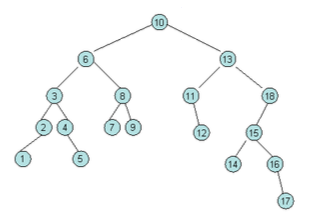
\includegraphics[scale=0.7]{images/mergesort}
\centering %centering the image
\caption{Merge sort}
\label{fig:mergesort}
\end{figure}
\end{boxed}

\begin{table}[H]
    %\caption{}
    \label{tab:bubblesort}
    \centering
    \begin{tabular}{|L{15em} | L{15em}|}
        \hline
        \rowcolor[HTML]{303F9F}
        \textbf{\textcolor{white}{Tilfelle}} & \textbf{\textcolor{white}{}}\\
        \rowcolor[HTML]{E6E6E6}
        Best case & $\theta(n lg n)$\\
        Average case & $\theta(n lg n)$\\
        \rowcolor[HTML]{E6E6E6}
        Worst case & $\theta(n lg n)$\\
        Minne & $\theta(n)$\\
        \rowcolor[HTML]{E6E6E6}
        In-place & Nei\\
        Stabil & Ja\\
        \rowcolor[HTML]{E6E6E6}
        Paralelliserbar & Ja\\
         \hline
    \end{tabular}
\end{table}

\subsubsection{HEAPSORT}
Her benytter vi oss igjen av deling av problemet slik at vi oppnår en god kjøretid. Heapsort er nok et eksempel på en sortering "in place".
\\\\
1. steg er bygging av heap. Dette består av å lage en såkalt "haug" av elementene først. En haug (eller en "heap") er et eksempel på en datastruktur. Det foregår slik at du setter elementene i et tre slik at ethvert element er det største av alle som er under det. Se figur \ref{fig:heapsort}. Dette innebærer blant annet at det øverste elementet er det største av alle de som er der. Algoritmen for å bygge opp en heap av en usortert liste med tall er nærmere forklart i kapittel 6.2 og 6.3 i Cormen, og går i korthet ut på at vi går gjennom alle indre noder og dytter dem nedover så langt som nødvendig. Noe som også lønner seg å få med seg fra boken er hvordan man kan lagre en heap direkte i et array i stedet for å lage en vanlig trestruktur.

\begin{figure}[H]
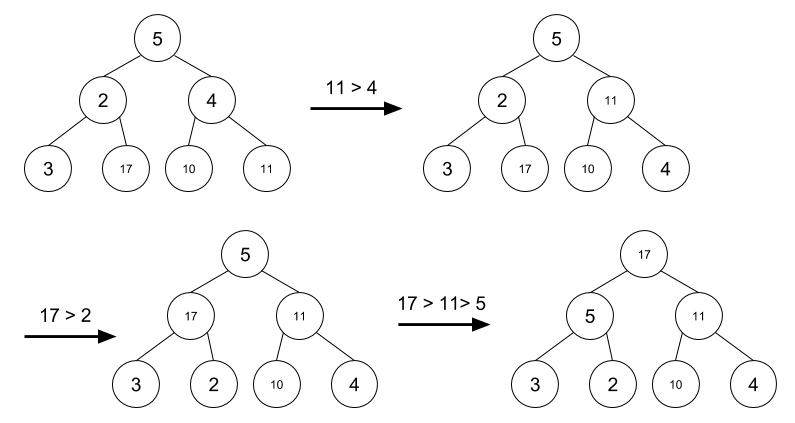
\includegraphics[scale=0.6]{images/heapsort}
\centering %centering the image
\caption{Heapsort}
\label{fig:heapsort}
\end{figure}

\noindent 2. steg er å sortere. Når haugen først er ferdig, går det fort å sortere. Bare plukk ut det øverste elementet i haugen, som er det største av samtlige. Deretter går der fort å ordne de resterende elementene i haugen igjen for deretter å plukke ut det største av dem igjen.

\begin{figure}[H]
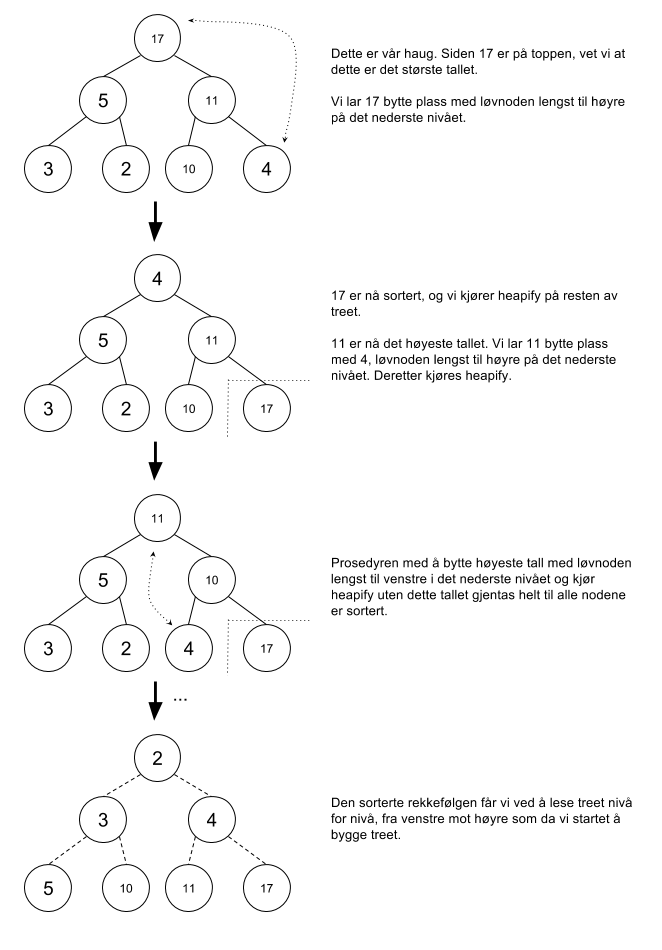
\includegraphics[scale=0.6]{images/heapsort2}
\centering %centering the image
\caption{Heapsortsortering}
\label{fig:heapsort2}
\end{figure}

\noindent Kjøretiden her er også \textbf{$\theta(n * log(n))$}. Det som er så fint med denne metoden er prinsippet med haugen. Dette kommer frem om du har med en \textbf{prioritetskø} å gjøre.

\begin{table}[H]
    %\caption{}
    \label{tab:bubblesort}
    \centering
    \begin{tabular}{|L{15em} | L{15em}|}
        \hline
        \rowcolor[HTML]{303F9F}
        \textbf{\textcolor{white}{Tilfelle}} & \textbf{\textcolor{white}{}}\\
        \rowcolor[HTML]{E6E6E6}
        Best case & $O(n lg n)$\\
        Average case & $O(n lg n)$\\
        \rowcolor[HTML]{E6E6E6}
        Worst case & $O(n lg n)$\\
        Minne & $\theta(1)$\\
        \rowcolor[HTML]{E6E6E6}
        In-place & Ja\\
        Stabil & Nei\\
        \rowcolor[HTML]{E6E6E6}
        Paralelliserbar & Nei\\
         \hline
    \end{tabular}
\end{table}

\subsubsection{BUILD-HEAP}

\subsubsection{MAX-HEAPIFY}

\subsubsection{BUILD-MAX-HEAP}
Build-max-heap går gjennom de resterende nodene av treet og kjører MAX-HEAPIFY på hver.

\begin{lstlisting}
    BUILD-MAX-HEAP(A)
	A.heap-size = A.length
	for i = ⌊A.length/2⌋ downto 1
		MAX-HEAPIFY(A,i)
\end{lstlisting}

\noindent Tiden som kreves av MAX-HEAPIFY når det kalles på en node av høyde $h$ er $O(h)$.

\begin{lstlisting}
    BUILDMAXHEAP(A)
        for i = A.length downto 2 do
	        exchange A[1] with A[i]
	        A.heapSize = A.heapSize - 1
	        MAX-HEAPIFY(A,1)
        end for
\end{lstlisting}

\subsubsection{EXTRACT-MIN}

\subsubsection{INCREASE-KEY}

\subsubsection{MAX-HEAP-INSERT}

\subsubsection{QUICKSORT}\\
Quicksort er en av de desidert mest populære sorteringene i bruk. Den bruker, som flettesortering, en form for \textit{splitt og hersk}-metode. Denne algoritmen kan deles i tre trinn:\newline

\noindent\textit{Partisjonér:} Velg ut et element i mengden du vil sortere. La oss kalle dette \textbf{pivotelementet} for $a$. Så deler vi mengden i to mindre mengder slik at alle elementer mindre eller lik $a$ danner den ene mengden, mens resten (som da er større enn $a$) danner den andre mengden.

\begin{boxed}
Anta at du har tallene 2 8 7 1 3 6 4
\newline \newline
Vi velger nå pivotlementet $a$ til å være det siste tallet 4. Tall som tilhører 1. partisjon, altså som er mindre eller lik $a$, understreker vi. De tallene som hører til 2. partisjon, overstreker vi. Algoritmen for splitting blir som følger:
\\\\
2 > 4, 2 tilhører 1. partisjon:\hfill \underline{2} 8 7 1 3 6 4\\

8 > 4, 8 tilhører 2. partisjon:\hfill \underline{2} $\overline{8}$ 7 1 3 6 4\\

7 > 4, 7 tilhører 2. partisjon:\hfill \underline{2} $\overline{8}$ $\overline{7}$ 1 3 6 4\\

1 < 4, 1 tilhører 1. partisjon:  1 bytter med 8\hfill \underline{2} \underline{1} $\overline{7}$ $\overline{8}$ 3 6 4\\

3 < 4, 3 tilhører 1. partisjon: 3 bytter med 7\hfill \underline{2} \underline{1} \underline{3} $\overline{8}$ $\overline{7}$ 6 4\\

6 > 4, 6 tilhører 2. partisjon:\hfill \underline{2} \underline{1} \underline{3} $\overline{8}$ $\overline{7}$ $\overline{6}$ 4
\newline\newline
Pivotelementet finner sin plass (4 bytter med 8), så partisjonen gir:
\begin{center}
2 1 3 4 7 6 8
\end{center}
\end{boxed}

\noindent Det finnes også andre måter å splitte på enn den i eksempelet.
\\\\
\textit{Hersk:} De to delmengdene sorteres ved å bruke quicksort igjen på hver av de to delene. Det er delle som kalles å gjøre et \textbf{rekursivt kall}.
\\\\
\textit{Kombinér:} Sett sammen delmengdene når du er ferdig med alle rekursive kall. Dette er lett, da Quicksort sorterer "in place".
\\\\
Dette kan virke greit, men hvordan velger man $a$, og når skal man avslutte de rekursive kallene? For å velge $a$, kan man ganske enkelt bare bruke den første verdien man har tilgjengelig. F.eks. om man har en liste med tall, bruker man det øverste tallet. Dette kan gå fint, men om tallmengden nesten er ferdig sortert vil denne metoden få en veldig stor kjøretid.
\\\\
Det er også et poeng at man ikke trenger å splitte helt til alle delmengdene bare består av ett enkelt element. På små datamengder er ikke Quicksort så veldig effektiv. Derfor er det ofte slik at når en delmengde har under et visst antall element, så sorterer man delmengden med en annen metode. Det er vanlig å sette grensen litt under 10, og så bruke sortering ved innsetting. Det samme gjelder mergesort.
\\\\
Gitt at vi klarer å velge elementet $a$ slik at den deler mengden i to nesten helt like store deler, vil Quicksort ha en kjøretid på \textbf{$\theta(n * log(n))$}. Dersom man kan velge $a$ helt tilfeldig vil den gjennomsnittlige kjøretiden være \textbf{$\theta(n * log(n))$}, mens verste tilfelle er $\theta(n^2)$. Derfor er det viktig å få randomisert når vi skal plukke ut $a$. Quicksort er raskere enn flettesortering og haugsortering selv om de to har både gjennomsnittlig og verste kjøretid på $\theta(n * log(n)$, eventuelt $O(n^2)$ og $\theta (n^2)$. Grunnen til det er at Quicksort har et veldig lite konstantledd.

\begin{lstlisting}
    function QUICKSORT(A,p,r)
    	if p < r then
    		q = PARTITION(A,p,r)
    		QUICKSORT(A,p,q - 1)
    		QUICKSORT(A.q + 1, r)
    	end if
    end function
\end{lstlisting}

\begin{table}[H]
    %\caption{}
    \label{tab:bubblesort}
    \centering
    \begin{tabular}{|L{15em} | L{15em}|}
        \hline
        \rowcolor[HTML]{303F9F}
        \textbf{\textcolor{white}{Tilfelle}} & \textbf{\textcolor{white}{}}\\
        \rowcolor[HTML]{E6E6E6}
        Best case & $\theta(n lg n)$\\
        Average case & $\theta(n lg n)$\\
        \rowcolor[HTML]{E6E6E6}
        Worst case & $\theta(n^2)$\\
        Minne & $\theta(lg n)$\\
        \rowcolor[HTML]{E6E6E6}
        In-place & Ja\\
        Stabil & Nei\\
        \rowcolor[HTML]{E6E6E6}
        Paralelliserbar & Nei\\
         \hline
    \end{tabular}
\end{table}

\subsubsection{PARTITION}

\begin{lstlisting}
    function PARTITION(A,p,r)
	    x = A[r]
    	i = p - 1
    	for j = p to r - 1 do
    		if A[j] $\leq$ x then
    			i = i + 1
    			exchange A[i] with A[j]
    		end if
    	end for
    	exchange A[i + 1] with A[j]
    	return i + 1
    end function
\end{lstlisting}

\subsubsection{RANDOMIZED-QUICKSORT}
Basert på designmetoden \textit{divide-and-conquer}. Bruker subrutinen PARTITION. Endrer kjøretid fra beste til verste tilfelle. Bruker en tilfeldig pivot for å unngå konsekvent worst case ved bestemte inputs (som f.eks. ferdig sortert liste).

\subsection{Sortering i lineær tid}
Hvis man kjenner til en del egenskaper ved mengden man skal sortere på forhånd kan man senke kjøretiden betraktelig.

\subsubsection{COUNTING SORT}
Anta at vi har en mengde men $n$ heltall med verdier fra 0 til $k$. Da kan vi rett og slett lage oss en liste fra 0 til $k$, og så setter vi hvert element inn på sin plass i listen. Sorteringen faller dermed ut av seg selv.

\begin{boxed}
Anta at vi har tretten tall mellom 1 og 9.
\begin{center}
3 9 8 9 4 1 5 4 7 8 2 4 7
\end{center}
Vi lager så en tabell hvor vi teller opp hvor mange vi har av hvert tall.

\begin{table}[H]
    \label{tab:tellesortering}
    \centering
    \begin{tabular}{|L{10em} | L{2em}|L{2em}|L{2em}|L{2em}|L{2em}|L{2em}|L{2em}|L{2em}|L{2em}|}
        \hline
        De mulige tall & 1 & 2 & 3 & 4 & 5 & 6 & 7 & 8 & 9\\
        \hline
        Antall av hvert tall & 1 & 1 & 1 & 3 & 1 & 0 & 2 & 2 & 2\\
         \hline
    \end{tabular}
\end{table}
Nå er det bare å hente ut den sorterte tallfølgen. Den blir da enkelt som følger:
\begin{center}
1 2 3 4 4 4 5 7 7 8 8 9 9
\end{center}
\end{boxed}

\noindent Kjøretiden til tellesortering avhenger av verdien til $k$. Hvis den ikke øker for mye i forhold til størrelsen, nærmere bestemt $k = O(n)$, så blir kjøretiden $\theta(k + n)$. Om du vet at alle (hel)tallene ligger i et bestemt område, f.eks. mellom 1 og 10, så er det tellesortering som er tingen. For om $k$ er konstant, så blir kjøretiden $\theta(n)$. Hvert element sjekkes for sin verdi én gang og settes i bås. Fungerer best når verdiene på tallene som sorteres ligger tett etterhverandre og $k$ ikke er for høy.

\begin{lstlisting}
    function COUNTINGSORT(A,B,k)
	    let C[0...k] be a new array
    	for i = 0 to k do
    		C[i] = 0
    	end for
    	for j = 1 to A.length do
    		C[A[j]] = C[A[j]] + 1
    	end for
    	for i = 0 to k do
    		C[i] = C[i] + C[i - 1]
    	end for
    	for j = A-length downto 1 do
    		B[C[A[j]]] = A[j]
    		C[A[j]] = C[A[j]] - 1
    	end for
    end function
\end{lstlisting}

\noindent Har kjøretid $O(n)$ i verste tilfelle, dersom $k = O(n)$ og $d = O(1)$.\\

\begin{boxed}
Gitt A = [3, 3, 1, 4, 4, 3, 1, 2, 3, 5]. Hvordan ser C[0...6] ut idet Counting-Sort(A, B, 6) returnerer?
\newline\newline
[0, 0, 2, 3, 7, 9, 10] \newline\newline  Tellesortering teller først forekomster, gjør så tellingene kumulative, og så dekrementerer disse under innsetting. Så tellingene til slutt tilsvarer altså hvor mange som er strengt mindre. F.eks. vil C[3] hvor mange verdier som er mindre enn 3. Her gis også enkelte andre svar noe uttelling.
\end{boxed}

\begin{table}[H]
    %\caption{}
    \label{tab:bubblesort}
    \centering
    \begin{tabular}{|L{15em} | L{15em}|}
        \hline
        \rowcolor[HTML]{303F9F}
        \textbf{\textcolor{white}{Tilfelle}} & \textbf{\textcolor{white}{}}\\
        \rowcolor[HTML]{E6E6E6}
        Best case & $\theta(n + k)$\\
        Average case & $\theta(n + k)$\\
        \rowcolor[HTML]{E6E6E6}
        Worst case & $\theta(n + k)$\\
        Minne & $\theta(n + k)$\\
        \rowcolor[HTML]{E6E6E6}
        In-place & Nei\\
        Stabil & Ja\\
        \rowcolor[HTML]{E6E6E6}
        Paralelliserbar & Nei\\
         \hline
    \end{tabular}
\end{table}

\subsubsection{RADIX SORT}\\
Når man skal sortere en mengde heltall (f.eks. i det vanlige titallsystemet) kan det være et smart triks å først sortere etter det mest signifikante sifferet (altså sifferet lengst til venstre), deretter det nest mest signifikante osv. til man er i mål. Det som ikke er så gunstig med dette er at når man er ferdig med å sortere på det første sifferet har man fått ti grupper som må sorteres videre hver for seg. Etter at hver av disse er sortert på det andre sifferet har man hundre grupper, og dette er det strevsomt å holde styr på.
\\\\
Radix-sortering bruker en lignende idé som er enda smartere. Du vil se at hvis man først sorterer etter det minst signifikante sifferet, vil man få sortert alle tallene uten det lille problemet som oppstår ve då ta fatt i det mest signifikante sifferet. For at dette skal fungere er det meget viktig at man bruker en stabil sorteringsalgoritme for å sortere på hvert siffer. Grunnen til dette er at når man sorterer på f.eks. sifferet nest lengst til høyre og støter på to tall med samme siffer på den plassen vil de to tallene beholde den innbyrdes rekkefølgen de hadde.
\\\\
Det er viktig at man bruker en lineær sorteringsalgoritme (som f.eks. tellesortering) som den indre algoritmen – hvis ikke forsvinner hele effektiviteten til radix sort. Hvis tallene er små, er kjøretiden til radix sort $\theta(n)$. Hvis du ikke har en konstant verdi for hvor store tallene kan være, er kjøretiden $\theta(nd)$, hvor $d$ er antall sifre i det største tallet. Merk at antall sifre i et tall $m$ er $\theta(lg m)$, så hvis du får oppgitt at ingen tall er større enn $m$, vet du at kjøretiden er $\theta(n lg m)$. 

\begin{figure}[H]
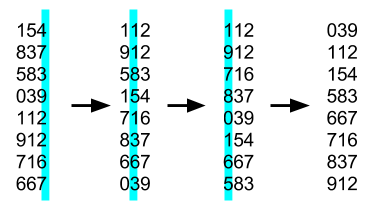
\includegraphics[scale=0.7]{images/radixsort}
\centering %centering the image
\caption{Radix sort}
\label{fig:radixsort}
\end{figure}

\noindent I Figur \ref{fig:radixsort} sorteres tallene etter sifrene i de fargede feltene fra forrige trinn. For eksempel blir 112 plassert høyere opp enn 154 under sorteringen på det midterste sifferet (siden 1 < 5), og på grunn av den stabile sorteringen vil 112 garantert forbli høyere plassert enn 154 også under sorteringen av sifferet lengst til venstre selv om de to tallene har samme siffer her (ustabile sorteringsalgoritmer kunne ha funnet på å bytte om rekkefølgen, siden det vanligvis er uinteressant hvilken rekkefølge like elementer står i – og 112 og 154 ser jo like ut når vi bare ser på sifferet lengst til venstre). Hvis to tall er like, så må det tallet som ligger bak det andre også gjøre det etter sorteringen. Hvis ikke blir det bare rot. Se på tallene 112 og 154. Etter andre sortering har vi funnet at 12 er mindre enn 54. Når så tallet 1 testes mot 1, så kan ikke vi tillate at deres rekkefølge etter sorteringen blir vilkårlig, for da risikerer vi å få at 154 er mindre enn 112.

\begin{lstlisting}
    function RADIXSORT(A,d)
    	for i = 1 to d do
    		Bruk Stabble sort til å sortere array A
    	end for
    end function
\end{lstlisting}

\begin{table}[H]
    %\caption{}
    \label{tab:bubblesort}
    \centering
    \begin{tabular}{|L{15em} | L{15em}|}
        \hline
        \rowcolor[HTML]{303F9F}
        \textbf{\textcolor{white}{Tilfelle}} & \textbf{\textcolor{white}{}}\\
        \rowcolor[HTML]{E6E6E6}
        Best case & $\theta(d(n + k))$\\
        Average case & $\theta(d(n + k))$\\
        \rowcolor[HTML]{E6E6E6}
        Worst case & $\theta(d(n + k))$\\
        Minne & $\theta(n + k)$\\
        \rowcolor[HTML]{E6E6E6}
        In-place & Nei\\
        Stabil & Ja\\
        \rowcolor[HTML]{E6E6E6}
        Paralelliserbar & Nei\\
         \hline
    \end{tabular}
\end{table}

\subsubsection{BUCKETSORT}
Bucketsort er nesten helt lik tellesortering, men bruker såkalte “bøtter” man putter tallene i. Trikset er at man lager "bøtter", eller tallintervaller, i listen i stedet for bare enkelttall. For eksempel [3,4) betyr at verdier større eller lik 3, men mindre enn 4 skal i bøtten. Når man har lagt alle tallene som skal sorteres inn i de tilhørende bøttene, sorterer man innholdet i hver bøtte etter en kjent og kjær sammenligningssortering, f.eks. insertion sort, og kombinerer det sorterte innholdet i bøttene til slutt.
\\\\
Forventet kjøretid for bøttesortering er $\theta(n)$. For å oppnå denne kjøretiden er tallene som sorteres nødt til å være uniformt fordelt (slik at det vil havne omtrent like mange tall i hver bøtte). I tillegg må antallet bøtter være omtrent like stort som antallet elementer som skal sorteres, for å unngå at for mange elementer må sorteres med sammenligningssorteringen.

\begin{lstlisting}
    function BUCKETSORT(A)
	    n = A.length
	    la B[0...n - 1] være et nytt array
	    for i = 0 to n - 1 do
	    	Gjør B[i] til en tom liste
	    end for
	    for i = 1 to n do
    		Sett inn A[i] i lista B[⌊nA[i]⌋]
    	end for
	    for i = 0 to n - 1 do
		    Sorter lista B[i] med INSERTIONSORT(B[i])
	    end for
	    Konkatiner listene B[0], B[1], …, B[n - 1] i rekkefølge
    end function
\end{lstlisting}

\noindent Bucket-Sort endrer kjøretid fra beste til verste tilfelle, og bruker ikke sammenligning.

\begin{boxed}
Lager bøtter for tallintervallene. Gitt tallene 29, 25, 3, 49, 9, 37, 21, 43. Lager bøtter for 0-9, her havner 3 og 9. 10-19 er tom. 20-29 får 21, 25 og 29. 30-39 får 37. 40-49 får 43 og 49.

\begin{figure}[H]
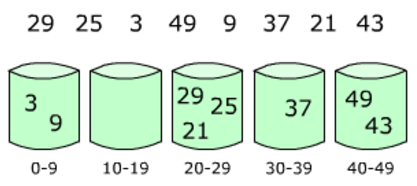
\includegraphics[scale=0.5]{images/bucketsort1}
\centering %centering the image
\caption{Bucketsort første trinn}
\label{fig:bucketsort1}
\end{figure}

Når dette så skal setter sammen til en sortert tallfølge hentes tallene opp fra bøttene igjen.

\begin{figure}[H]
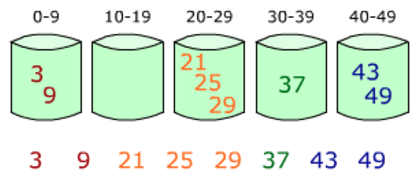
\includegraphics[scale=0.5]{images/bucketsort2}
\centering %centering the image
\caption{Bucketsort andre trinn}
\label{fig:bucketsort2}
\end{figure}

Tallfølgen blir da til slutt 3,9, 21, 25, 29, 37, 43, 49.
\end{boxed}



\subsubsection{SELECTION SORT}
Denne metoden er en av de enkleste å sortere på, og en av de tregeste. For hver iterasjon finner man det største usorterte elementet, og bytter ut med det siste usorterte elementet. Denne algoritmen er veldig treg. Det vil ta $n$ operasjoner for å finne det største elementet, og siden dette gjøres $n$ ganger (ved hver iterasjon). Dermed får man kjøretiden $O(n^2)$. Bruker sammenligning.

\begin{boxed}
Gitt tallfølgen 8, 5, 2, 6, 9, 3, 1, 4, 0, 7. Vi begynner på plass null og ser hva verdien er der; 8. Går gjennom hele rekken for å finne noe lavere. 5 er lavere, så vi holder av den. 2 er lavere, 1 enda lavere, 0 lavest. 0 og 8 bytter plass. Tallfølgen er nå 0, 5, 2, 6, 9, 3, 1, 4, 8, 7. Ser på plass en. Denne er 5. Leter etter noe mindre. 2 er mindre, 1 er mindre. Bytter om 5 og 1. Tallene er nå 0, 1, 2, 6, 9, 3, 5, 4, 8, 7. Ser på plass to; 2. Ingen mindre, ok. Ser på plass tre; 6. 3 er mindre. Bytter 6 og 3. 0, 1, 2, 3, 9, 6, 5, 4, 8, 7. Ser så på plass fire; 9. 6 er mindre, 5 er mindre, 4 er mindre. 4 og 9 bytter plass. 0, 1, 2, 3, 4, 6, 5, 9, 8, 7. Ser på plass fem: 6. 5 er mindre. Bytter plass. 0, 1, 2, 3, 4, 5, 6, 9, 8, 7. Plass seks; 6. 0, 1, 2, 3, 4, 5, 6, 9, 8, 7. Ok. Plass syv; 9. 8 er mindre, 7 er mindre. Bytter 9 og 7. 0, 1, 2, 3, 4, 5, 6, 7, 8, 9. Plass åtte; 8. Ok. Plass ni; 9. Ok.
\end{boxed}

\begin{table}[H]
    %\caption{}
    \label{tab:selectionsort}
    \centering
    \begin{tabular}{|L{15em} | L{15em}|}
        \hline
        \rowcolor[HTML]{303F9F}
        \textbf{\textcolor{white}{Tilfelle}} & \textbf{\textcolor{white}{}}\\
        \rowcolor[HTML]{E6E6E6}
        Best case & $\theta(n^2)$\\
        Average case & $\theta(n^2)$\\
        \rowcolor[HTML]{E6E6E6}
        Worst case & $\theta(n^2)$\\
        Minne & $\theta(1)$\\
        \rowcolor[HTML]{E6E6E6}
        In-place & Ja\\
        Stabil & Nei\\
        \rowcolor[HTML]{E6E6E6}
        Paralelliserbar & Nei\\
         \hline
    \end{tabular}
\end{table}

\subsubsection{SELECT}
% https://www.youtube.com/watch?v=9K8L1vjAmk0
Basert på designmetoden divide-and-conquer. Har kjøretid $O(n)$ i verste tilfelle, dersom $k = O(n)$ og $d = O(1)$. Bruker subrutinen PARTITION.
\\\\
SELECT gjør det samme som RANDOMIZED-SELECT – den bare velger pivot litt smartere. Den gjør det ved å først dele inn tabellen i grupper og å finne medianen i hver av disse (vha. INSERTION-SORT), og så bruker den SELECT rekursivt for å finne medianen av disse medianene. Denne medianen av medianer brukes så som pivot på samme måte som i RANDOMIZED-SELECT, og vi fortsetter rekursivt i riktig halvdel.


\subsubsection{RANDOMIZED-SELECT}
Basert på designmetoden divide-and-conquer. Bruker subrutinen PARTITION. Endrer kjøretid fra beste til verste tilfelle.

\subsubsection{TOPOLOGICAL-SORT}
%FYLL INN HER
Topologisk sortering bruker en DAG til å finne en rekkefølge gjennom alle elementene i grafen. Det tillates ikke sykler. Man begynner i noden som ikke har noen kanter inn til seg.

\begin{lstlisting}
    function TOPOLOGICALSORT(G)
    	DFS(G) to compute finish times v.f for each vertex v.
    	as each vertex is finished, insert it onto the end of the list
    	return the list of vertices
    end function
\end{lstlisting}

\subsection{Finne $i$-te verdi}
Hvordan skal man gå frem hvis man i en tallmengde vil finne den $i$-te største (eller den $i$-te minste) verdien? Anta at man sorterer med sammenligning. Da har vi lært at beste kjøretid er $\theta(n * log(n))$. En annen mulighet er å finne største verdi for deretter å eliminere denne. Ved å fortsette slik finner man det nest største, tredje største osv. helt til man kommer til det $i$-te største. Men om det $i$-te største ligger rundt midten, så er vi nødt til å finne største tall et antall ganger som er proporsjonalt med antallet tall. Dermed blir kjøretiden $\theta(ni)$, som i verste tilfelle er $\theta(n^2)$, som er dårligere enn det vi fikk i sted. Er det mulig å finne det $i$-te største elementet med en kjøretid på $\theta(n)$? Vi ser lett at dette gjelder for det største elementet. Også for det $i$-te største er svaret ja.
\\\\
Trikset er å bruke partisjoneringsmetoden fra \textbf{quicksort}. Vi velger et tilfeldig element som pivotelement, kall den \textit{p}, og lager to delmengder av den opprinnelige mengden vår. Dermed har vi at hvis posisjonen til \textit{p} er mindre enn \textit{i}, så holder det å lete i øvre halvdel, og er den mindre leter vi i nedre halvdel. Hvis posisjonen til \textit{p} er akkurat \textit{i}, så er \textit{p} det elementet vi leter etter. I quicksort kjørte vi rekursive kall på begge delmengder. Her gjør vi et rekursivt kall bare i den ene delmengden, så kjøretiden for denne metoden er $\theta(n)$ hvis man har en god strategi for valg av pivotelement. Det er ikke så vanskelig å se for seg: først partisjonerer man hele listen, så halve listen, osv. Summen av rekken $n$ + $\frac{n}{2}\)$ + \frac{n}{4}\) + $\frac{n}{8}\)$ + ... er $2n$. 

\begin{boxed}
Anta at vi har tallfølgen 2 8 7 1 3 6 4
\newline\newline
Vi ønsker å finne det tredje minste tallet. Med 4 som pivotelement har vi allerede at første splitt gir oss:
\begin{center}
2 1 3 4 7 6 8
\end{center}
Alle verdier til venstre for 4 er mindre eller lik, alle til høyre er større. Det vi nå vet, er at 4 er det fjerde minste elementet. Dermed kan vi se bort fra tallene 4, 7, 6 og 8, og vi står igjen med å finne det tredje minste tallet av:
\begin{center}
2 1 3
\end{center}
Velger vi så 2 som pivotelement, så gir splitten oss:
\begin{center}
1 2 4
\end{center}
2 er det nest minste elementet, vi kan se bort fra det og tallet 1. Dermed er det bare tallet 3 igjen, og det er det minste tallet i følgen vår.
\end{boxed}

\subsection{Hashing}
Venligvis brukes \textbf{direkte adressering} når man skal slå opp på elementet på plass nummer \textit{i} i en array, noe som går på konstant tid. Dette fungerer så lenge vi har råd til å ha en liste som har én posisjon for hver mulig verdi. Men dette kan gi mange ubrukte plasser. Hvis man for eksempel vil lagre data om personer slik at man kan gjøre oppslag på fødselsnumre, trenger man et array med over 30 milliarder plasser for å kunne gjøre direkte oppslag på fødselsnumrene. Siden 11 sifre er i bruk, vil mesteparten av den enorme plassen som er satt av til arrayet være bortkastet. For å ikke sløse slik med plassen, benytter man seg av \textbf{hashing}. Dette er ikke så ulikt prinsippet for bøttesortering. Man kan tenke seg at en hashtabell består av en mendge bøtter, og i hver av bøttene er det rom for et par posisjoner fra listen. Slik vil mye plass kunne spares dersom man klarer å lage hashtabellen liten. Men det er en risiko for at det faller flere verdier i en og samme bøtte. Det er dette som kalles \textbf{kollisjoner}.
\\\\
For å få bukt med kollisjoner, er det et godt triks å bruke \textbf{lenkede lister}. Men, da risikerer man at noen av listene blir veldig lange – hvis man er veldig uheldig vil alt ende opp i samme liste. Et annet gyllent triks er det som kalles \textbf{åpen adressering}. Enkelt sagt vil dette si at hvis man vil legge til et element og dennes plass er opptatt, så legger man rett og slett elementet inn i den første ledige plassen lenger bort i tabellen. Dessverre er det en del problemer som kan oppstå, så dette er en litt komplisert affære.
\\\\
Et svert aktuelt spørsmål er hvordan man skal lage hashtabellen. Selve tabellen er bare en vanlig array. Man snakker om en hash-funksjon \textit{h} som tilordner enhver posisjon i listen til en posisjon i hashtabellen. Men denne må velges med kløkt, så elementene blir spredd mest mulig.

\begin{itemize}
    \item \textbf{Divisjonsmetoden}\\
La \textit{k} være nummeret til posisjonen i listen, og la \textit{m} være antallet plasser i hashtabellen. Da kan man sette hashfunksjonen til å ta resten av \textit{k} når det deles på \textit{m}. Altså:
\begin{center}
$h(k) = k$ mod $m$
\end{center}
hvor tabellstørrelsen \textit{m} må velges med omhu for at resultatene skal bli gode. Et godt valg er å la \textit{m} være et primtall og holde det langt unna en potens av tallet 2.
\item \textbf{Multiplikasjonsmodellen}\\
Denne metoden går i to trinn. Først multipliserer vi \textit{k} med et tall \textit{A} som ligger mellom 0 og 1. Deretter tar vi desimalene (eller resten av flyttallsdivisjonen med tallet 1) og ganger med en verdi \textit{m}, og runder av nedover. Matematisk blir dette:
\begin{center}
$h(k) = \lfloor m((kA) mod 1) \rfloor$
\end{center}
 \end{itemize}

\noindent Når det gjelder kjøretider til hashing så går det stort sett fort. Å slå opp i et vanlig array går på $O(1)$ tid. Hashing går som oftest like raskt i praksis, med $O(1)$ i gjennomsnittlig kjøreitd. Konstantleddet er dog større i hashing, fordi vi må bruke hashfunksjonen for å regne ut plasseringen og kanskje håndtere kollisjoner. Husk at hvis hashfunksjonen er sårlig stilt slik at veldig mange elementer havner på samme sted i hashtabellen (og vi fikser kollisjoner med en lenket liste) så vil hashingen oppøre seg nesten som en lenket liste og kjøretiden blir $O(n)$ i verste tilfelle. Det finnes bedre metoder, blant annet \textbf{lineær probing} og \textbf{kvadratisk probing}, som står i Cormen. \textbf{Perfekt hashing} gir enda bedre resultater i visse situasjoner, men akkurat det er hardcore og vi lar det ligge.

 
\subsection{Søking}

\subsubsection{Brute force}

\subsubsection{Binærsøk}
Et binært søketre er et tre som tilfredsstiller binært-søketre-egenskapen.

\begin{table}[H]
    %\caption{}
    \label{tab:binaert}
    \centering
    \begin{tabular}{|L{10em} | L{10em}| L{10em}|}
        \hline
        \rowcolor[HTML]{303F9F}
        \textbf{\textcolor{white}{Operasjon}} & \textbf{\textcolor{white}{Average}} & \textbf{\textcolor{white}{Worst}}\\
        \rowcolor[HTML]{E6E6E6}
        Plass (bit) & $O(log n)$ & $O(n)$\\
        Søk & $O(log n)$ & $O(n)$ \\
        \rowcolor[HTML]{E6E6E6}
        Sett inn & $O(log n)$ & $O(n)$ \\
        Slett & $O(log n)$ & $O(n)$ \\
         \hline
    \end{tabular}
\end{table}

\begin{boxed}
Hvis du setter verdiene 1, 2, 9, 5, 10, 7, 6, 4, 8 og 3 inn i et tomt binærtre (én etter én, i oppgitt rekkefølge), hva blir høyden til treet (antall kanter i den lengste stien fra rota til en løvnode)?
\newline\newline
5
\end{boxed}

\begin{boxed}
La $x$ være en gitt node i søketreet. Hvis $y$ er en node i det venstre subtreet til $x$ må $y$ sin verdi være mindre eller lik ($\leq$) $x$ sin verdi. Tilsvarende for høyre subtre. Her må $y$ sin verdi være større enn eller lik ($\geq$) $x$ sin verdi.

\begin{figure}[H]
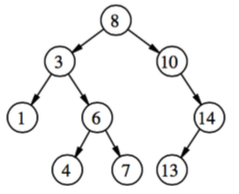
\includegraphics[scale=0.7]{images/binaer}
\centering %centering the image
\caption{Binært tre}
\label{fig:binaer}
\end{figure}
\end{boxed}

